\chapter{Experimente und Ergebnisse}
In diesem Kapitel werden verschiedene Experimente mit dem FPGA durchgeführt. Zunächst wird gemessen, Wie viel Zeit pro trainiertem Perzeptron für das Training und die Voraussagen auf dem FPGA und einer Implementierung auf dem Hostsystem aufgewendet werden muss. Hierbei wird das Programm auf dem Hostsystem nicht parallelisiert. 
Dann werden beispielhaft Trainingsvorgänge mit verschiedenen Datensätzen durchgeführt, um die Genauigkeit der Vorhersagen zu überprüfen und Ergebnisse der Testvorgänge zu präsentieren.\\
Es werden für die Experimente die Datensätze MNIST \cite{MNIST}, und verwendet.\\
Die Features $\vec f$ des jeweiligen Datensatzes wurden normalisiert, so dass $\forall f \in \vec f\text{ . } f \in [0,1]$. 
\section{Regularisierung}
Mit dem MNIST Datensatz wurden verschiedene Testzyklen zur Regularisierung durchgeführt. Für die Ergebnisse ist der Datentyp, soweit nicht anders vermerkt, auf eine Fixkommazahl mit einem Vorzeichen-, 4 Vorkommastellen- und 11 Nachkommastellenbits eingestellt. Ein Trainingsdurchlauf mit 200 Variablen und 100 Wiederholungen führte zu folgenden Ergebnissen: \\\\
\begin{tabularx}{\textwidth}{p{0.16\textwidth}|r|r|r|r|r}
Perceptron & Regularisierungsrate & Lernrate & Batch & Methode & Genauigkeit\\
\hline
a & 0.0 & 0.100098 & 1 & keine & 95.43\%\\
\hline
b & 0.007812 & 0.100098 & 1 & L2 & 95.75\%\\
\hline
c & 0.009766 & 0.100098 & 1 & L2 & 95.75\%\\
\hline
d & 0.5 & 0.100098 & 1 & L2 & 89.9\%\\
\hline
e & 0 & 0.100098 & 1 & L1 & 95.43\%\\
\hline
f & 0.000977 & 0.100098 & 1 & L1 & 95.43\%\\
\hline
g & 0.004883 & 0.100098 & 1 & L1 & 94.38\%\\
\hline
h & 0.009766 & 0.100098 & 1 & L1 & 93.38\%\\
\end{tabularx}\\\\
Hierbei wurde der Datensatz so angepasst, dass alle Variablen die die Ziffer "`3"' darstellen mit "`trifft zu"' und alle anderen Variablen mit "`trifft nicht zu"' markiert wurden.\\
Nach dem Auswerten der Koeffizienten sind die Einflüsse der Regularisierungsmethoden auf das gelernte Modell deutlich sichtbar. Die Ridge Regression erzielte bei diesem Versuch die besten Ergebnisse, was aufgrund der Daten nicht besonders überraschend war. Da MNIST aus 28x28 Pixeln in Schwarz-Weiß Werten besteht und diese eine handgeschriebene Ziffer repräsentieren war anzunehmen dass es nur wenige Features gibt  welche für das Ergebnis irrelevante Ausprägungen bieten. Demnach ist die LASSO Methode für diesen Datensatz nicht gut geeignet. Die Ridge Regression kann, mit ausreichend kleinem $C$, die Koeffizienten, die zu starke Auswirkungen auf das Modell haben reduzieren, sodass einem Overfitting entgegengewirkt wird. Allerdings hat der gewonnene Genauigkeitswert nur geringfügig zugenommen.\\
Zeichnet man die Koeffizienten als Graphen auf kann man die Auswirkung der Regularisierung auf die Regression deutlich erkennen. In den nachfolgenden Abbildungen 5.1, 5.2 und 5.3 werden diese Graphen dargestellt. Die Koeffizienten sind hierbei die Ergebnisse der obigen Trainingsdurchlaufs.
\begin{figure}[ht]
\centering
  	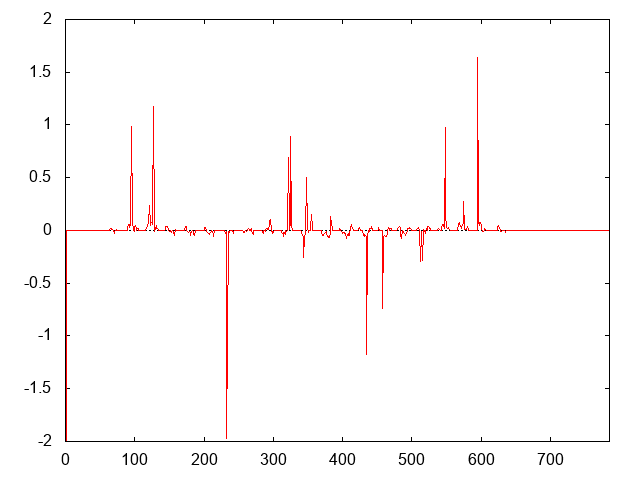
\includegraphics[scale=0.5]{bilder/features7}
  	\caption{L1 Regularisierung}
\end{figure}
\begin{figure}[ht]
\centering
  	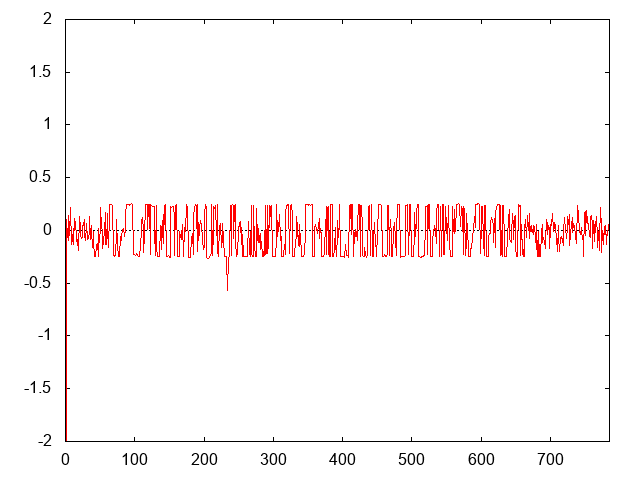
\includegraphics[scale=0.5]{bilder/features2}
	\caption{L2 Regularisierung}
\end{figure}
\begin{figure}[ht]
\centering
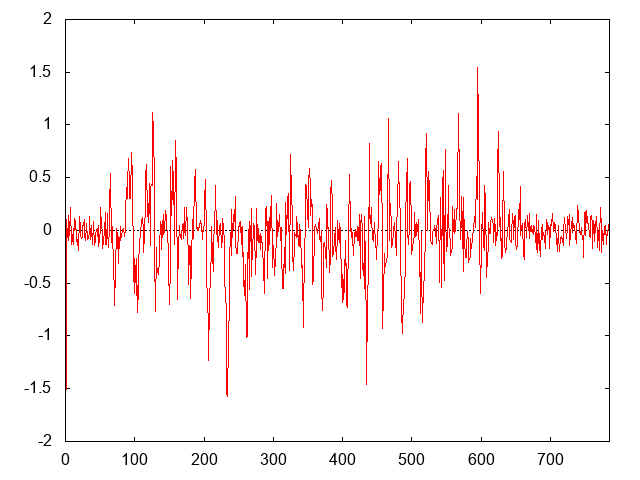
\includegraphics[scale=.5]{bilder/features0}
\caption{Logistische Regression ohne Regularisierung}
\end{figure}\newpage
Bei der Verarbeitung von Bilddaten gibt es den großen Vorteil, dass sich die Koeffizienten selbst als Bild interpretieren lassen. In der ersten Zeile der folgenden Grafiken (Abbildung 5.4, 5.5, 5.6) wurden die Koeffizienten unverändert interpretiert, sodass negative Werte keinen Farbunterschied hervorrufen. Es sind auf den Bildern nur die Koeffizienten zu sehen die einen positiven Einfluss auf die Ausgabe haben, da sie die Features repräsentieren die das Vorhandensein einer Linie belohnen. Der Verlauf ist von Schwarz (keine oder negative Auswirkung) bis hin zu Weiß (positive Auswirkung).\\
In der zweiten Zeile (Abbildung 5.7, 5.8, 5.9) sind die Koeffizienten normalisiert worden, sodass die kleinste Ausprägung 0 und die größte Ausprägung 1 darstellen. Es wird also auch der negative Einfluss der Features berücksichtigt, also derer, die das Vorhandensein einer Linie bestrafen.\newpage
\begin{figure}[ht]
\centering
	\begin{minipage}[b]{.25\linewidth}
  		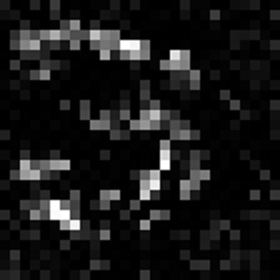
\includegraphics[scale=0.7]{bilder/l0_3}
  		\caption{ohne Regularisierung}
  	\end{minipage}
  	\hspace{.05\linewidth}% Abstand zwischen Bilder
  	\begin{minipage}[b]{.25\linewidth}
  		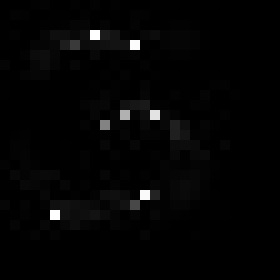
\includegraphics[scale=0.7]{bilder/l1_3}
		\caption{L1 \\Regularisierung}
	\end{minipage}
	\hspace{.05\linewidth}% Abstand zwischen Bilder
	\begin{minipage}[b]{.25\linewidth}
  		
\includegraphics[scale=0.7]{bilder/l2_3}
  		\caption{L2 \\ Regularisierung}
  	\end{minipage}
	\begin{minipage}[b]{.25\linewidth}
  		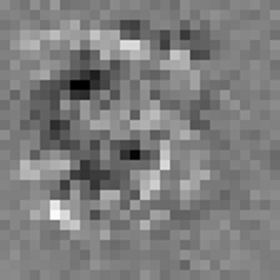
\includegraphics[scale=0.7]{bilder/l0_3_g}
  		\caption{ohne Reg. normiert}
  	\end{minipage}
  	\hspace{.05\linewidth}% Abstand zwischen Bilder
  	\begin{minipage}[b]{.25\linewidth}
  		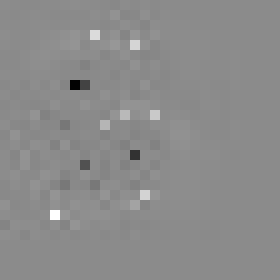
\includegraphics[scale=0.7]{bilder/l1_3_g}
		\caption{L1 normiert}
	\end{minipage}
	\hspace{.05\linewidth}% Abstand zwischen Bilder
	\begin{minipage}[b]{.25\linewidth}
  		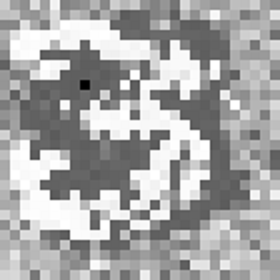
\includegraphics[scale=0.7]{bilder/l2_3_g}
  		\caption{L2 normiert}
  	\end{minipage}
\end{figure}
Die MNIST Daten sind so auf den angezeigten Bildausschnitt normiert, das der Schwerpunkt der Pixel mit einer gezeichneten Linie zur Bildmitte hin verschoben ist. Die "`3"' zu Beispiel, wie in den Graphiken oben zu sehen, ist nach oben links im Bild verzogen, die "`9"' hingegen nach unten links.
Da sich nicht alle Ziffern perfekt überlappen gibt es für die L1 Regularisierung sehr wenige Koeffizienten, die auf 0 gesetzt werden können. Demnach hat diese Regularisierungsmethode nur mit kleiner Gewichtung eine positive Auswirkung auf das Endergebnis. In den folgenden Graphiken zeigt sich deutlich, dass eine Ausdünnung der Koeffizienten schon bei sehr kleine Hyperparametern C zu schlechteren Vorhersagen führt.
Dennoch ist die Wahl dieser Methode, sofern C richtig gewählt wird, durchaus berechtigt, denn zum einen liegt eine kleine Verbesserung vor, zum anderen können zumindest die für die Entscheidung ausschlaggebenden Features isoliert werden.\newpage
\begin{figure}[ht]
\centering
	\begin{minipage}[b]{.45\linewidth}
  		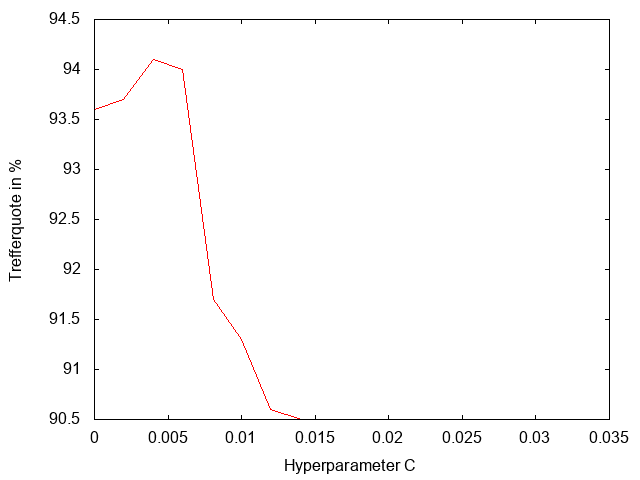
\includegraphics[scale=0.4]{bilder/pareto_l1_MNIST}
  		\caption{L1 nach C mit Fixkomma}
  	\end{minipage}
  	\hspace{.05\linewidth}% Abstand zwischen Bilder
  	\begin{minipage}[b]{.45\linewidth}
  		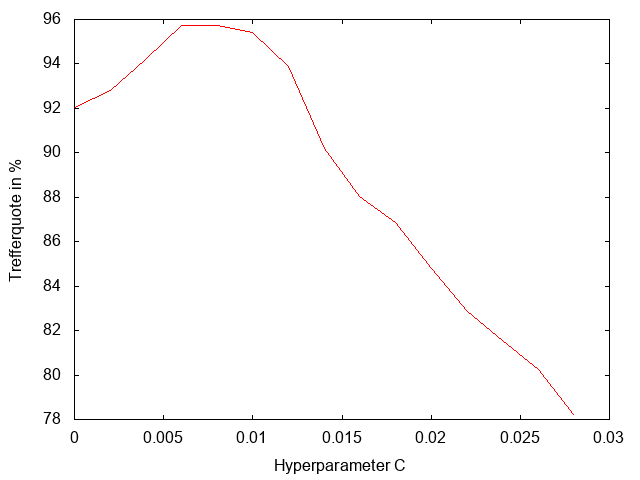
\includegraphics[scale=0.4]{bilder/pareto_l1_float_single}
		\caption{L1 nach C mit Float}
	\end{minipage}
	\hspace{.05\linewidth}% Abstand zwischen Bilder
\end{figure}
\begin{figure}[ht]
\centering
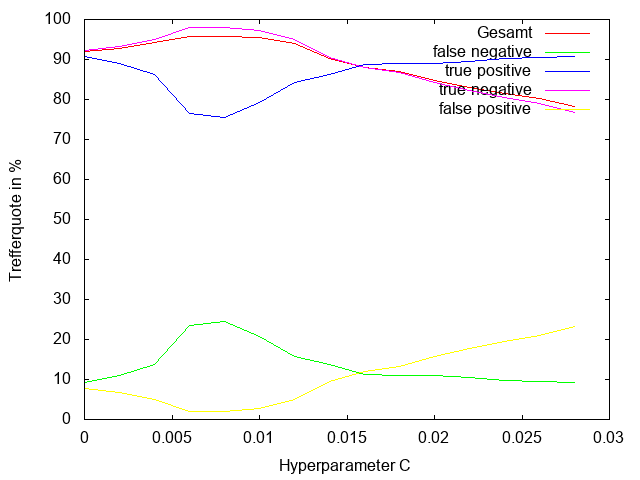
\includegraphics[scale=.7]{bilder/pareto_l1_float}
\caption{L1 Regularisierung mit Float}
\end{figure}
Im Gegensatz dazu kann die L2 Regularisierung die Ergebnisse mit etwas größerem Hyperparameter C geringfügig verbessern, sodass bei der Wahl der Regularisierungsmethode auf Ridge Regression zurückgegriffen werden sollte. Sowohl die Vorhersagen bei der L1- als auch bei der L2 Regularisierung klassifizieren mehr Variablen mit Bezeichnung 0 korrekt als negativ, aber es werden auch mehr Variablen mit Bezeichnung 1 fälschlicherweise als negativ eingeordnet. 

\begin{figure}[ht]
\centering
	\begin{minipage}[b]{.45\linewidth}
  		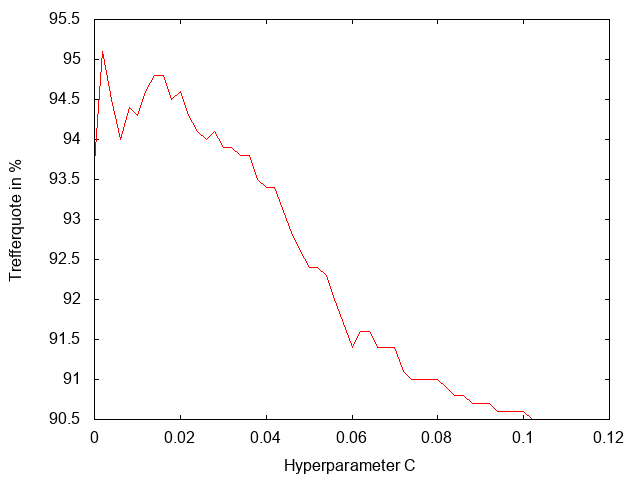
\includegraphics[scale=0.4]{bilder/pareto_l2_MNIST}
  		\caption{L2 nach C mit Fixkomma}
  	\end{minipage}
  	\hspace{.05\linewidth}% Abstand zwischen Bilder
  	\begin{minipage}[b]{.45\linewidth}
  		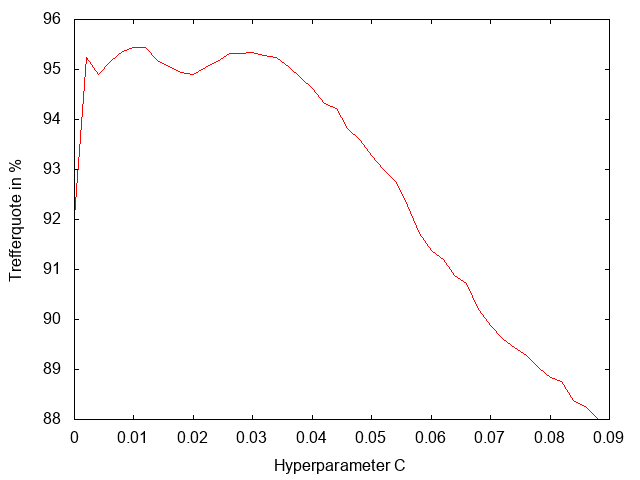
\includegraphics[scale=0.4]{bilder/pareto_l2_float_single}
		\caption{L2 nach C mit Float}
	\end{minipage}
	\hspace{.05\linewidth}% Abstand zwischen Bilder
\end{figure}
\begin{figure}[ht]
\centering
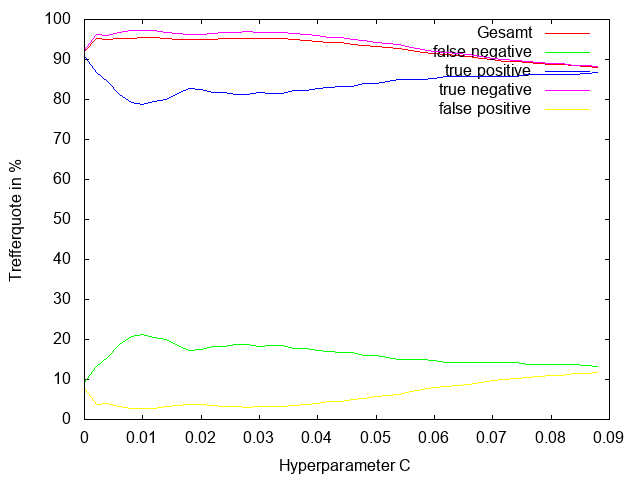
\includegraphics[scale=.7]{bilder/pareto_l2_float}
\caption{L2 Regularisierung mit Float}
\end{figure}\newpage

\section{Festkomma- und Gleitkommazahl}
Die Wahl einer Festkommazahl im Gegensatz zu einer Gleitkommazahl liegt durch deren Eigenschaften von Beginn an nahe. Berechnungen mit Fixkommazahlen sind ressourcenschonender und schneller als Gleitkommaberechnungen, bei denen die Anzahl Bits für die Vor- und Nachkommastelle mit jeder Zahl variieren können. zudem können auf der verwendeten 32-Bit Schnittstelle von Xillybus zwei Fixkommazahlen mit der Länge von 16 oder weniger Bits gleichzeitig übertragen werden. Dies sollte die Übertragungszeit für die Daten an den FPGA halbieren. \\
Überraschenderweise sind aber die Fixkommazahlen auf dem FPGA deutlich Ressourcenabhängiger als die Gleitkommazahlen. eine Belegung des FPGA mit 16 Perceptrons erzielt für Fixkomma- und Gleitkommazahlen jeweils folgende Auslastungen:\\\\
Fixkommazahl:\\\\

\begin{tabularx}{.6\textwidth}{p{0.16\textwidth}|r|r|r}
Bauteil & Benutzt & Gesamt & Auslastung \\
\hline
LUT & 120478 & 133800 & 90.04\%\\
\hline
LUTRAM & 685 & 46200 & 1.48\%\\
\hline
FF & 757423 & 267600 & 28.18\%\\
\hline
BRAM & 37 & 365 & 10.14\%\\
\hline
DSP & 400 & 740 & 54.05\%\\
\hline
I/O & 5 & 400 & 1.25\%\\
\end{tabularx}\\\\
Gleitkommazahl:\\\\

\begin{tabularx}{.6\textwidth}{p{0.16\textwidth}|r|r|r}
Bauteil & Benutzt & Gesamt & Auslastung \\
\hline
LUT & 82816 & 133800 & 61.90\%\\
\hline
LUTRAM & 1586 & 46200 & 3.43\%\\
\hline
FF & 81956 & 267600 & 30.63\%\\
\hline
BRAM & 61 & 365 & 16.67\%\\
\hline
DSP & 400 & 740 & 54.05\%\\
\hline
I/O & 5 & 400 & 1.25\%\\
\end{tabularx}\\\\

Durch diese doch deutlich abweichenden Werte gelingt es mit Gleitkommazahlen 24 Perceptrons auf dem FPGA parallel laufen zu lassen.
Der eventuelle Zeitverlust durch die größeren Zahlen wird hierdurch ausgeglichen. \\ 
Auch auf dem Hostrechner laufen die Programme unter Gleitkommazahlen schneller und flüssiger als mit Festkommawerten. Eine mögliche Erklärung dafür ist, dass die Werte aus den Datensets in Gleitkommazahlen vorliegen und erst in Festkommazahlen umgerechnet werden müssen. Auch die Einstellungen $AP\_SAT\_SYM$ und $AP\_RND\_CONV$, obgleich sie wichtig für die Funktionalität auf dem FPGA sind, brauchen bei jeder Belegung und Berechnung Rechenzeit um die Direktiven auf die Zahl anzuwenden. Zusätzlich ist es auf dem FPGA bei größeren Batchgrößen die Berechnung der Summe der Kostenfunktionen in Gleitkommazahlen durchzuführen, wodurch eine weitere Umrechnung nötig ist. Beispielweise ist bei einer Batchgröße von 60 der maximale Wert, den ein Hilfskoeffizient annehmen kann auch 60 und damit größer als das Maximum von \textit{ap\_fixed(3, 16)}. Es bleibt also nur die Wahl zwischen dem Umrechnen in Gleitkommazahlen zum aufaddieren der Hilfskoeffizienten oder dem Dividieren der der Hilfskoeffizienten bei jeder Berechnung durch die Batchgröße. Auch die Zweite Möglichkeit kann dazu führen dass der Wert nicht mehr korrekt dargestellt werden kann und zu 0 gerundet wird. 